\section{Сценарий Ландау-Хопфа}

\begin{frame}
\frametitle{Мультипликатор}
    При $\R > R_{\text{кр}}$ найдём решения для:
    $$
        \vc{v} = \vc{v_0} + \vc{v}_2.
    $$
    Решение будем искать в виде:
    $$
        \vc{v}_2 = \Pi(\vc{r}, t) e^{-i\omega t}, \text{ где }  \mu \equiv e^{-i\omega t} \text{ -- мультипликатор.}
    $$
    Потеря устойчивости происходит при $\mu \gtrsim 1$. 
\end{frame}


\begin{frame}
\frametitle{<<Рождение>> двумерного тора}
    Пусть $\mu = \exp{\left(\pm 2 \pi \alpha i\right)}$, где $\alpha \in \mathbb{R} \setminus \mathbb{Q}$.
    \begin{figure}
        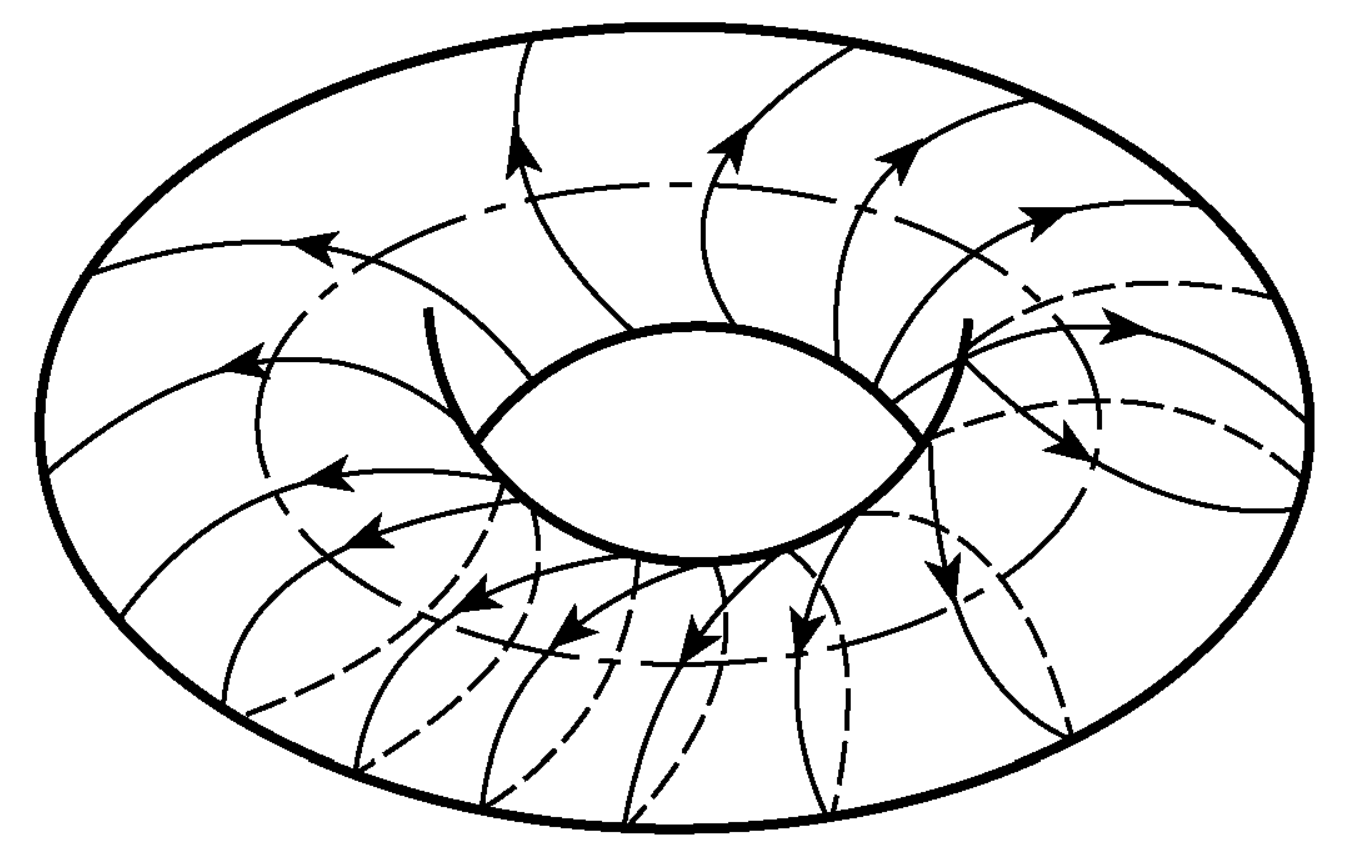
\includegraphics[width=0.4\linewidth]{img/tor.png}
    \end{figure}
Геометрическим образом этого движения в пространстве состо-
яний служит траектория в виде незамкнутой намотки на двумерном
торе.

\end{frame}

\begin{frame}
\frametitle{Причины}
    
\textbf{Предположим}, что при $\R \uparrow$ будут последовательно появляться новые несоизмеримые периоды.

\phantom{42}

2D тор $\leadsto$ 3D тор $\leadsto$ $\ldots$ $\leadsto$ $N$D тор $\leadsto$ $\ldots$

\phantom{42}

Интервалы между числами $\R_{\text{кр}}$ $\downarrow$, \\
появляющиеся движения имеют все меньшие масштабы.

\phantom{42}

Движение приобретает сложный характер — \textbf{турбулентный}.

\end{frame}

\begin{frame}
\frametitle{Реализация}

Общий вид функции:
$$
    \vc{v}(\vc{r}, t) = \sum \vc{A}_{p_1 p_2 \ldots p_N} (\vc{r}) \exp \left(-i \sum_{i=1}^{N} p_i \varphi_i \right),
$$

Интересное нам время:
$$
    t = \frac{\alpha - \beta_1}{\omega_1} + 2 \pi s \frac{1}{\omega}.
$$

Значение $\varphi_2$:
$$
\varphi_2 = \beta_2 + \frac{\omega_2}{\omega_1}\left(\alpha - \beta_1 + 2 \pi s\right).
$$


Время возврата, растет с увеличением $N$ и становится столь большим, что никакого следа периодичности не остается.    


\end{frame}


\begin{frame}
\frametitle{Проблема (синхронизация колебаний)}
\begin{itemize}
    \item[1)] Пусть возмущенное решение содержит 2 независимые $\omega$.
    \item[2)] Возмущение на $\omega_1$ $\in U(\R_{\text{кр2}})$ интенсивно  \\
$\Rightarrow$ возмущение на $\omega_1$ $\equiv \const$ при $\R \in U(\R_{\text{кр2}})$.
    \item[3)] В некотором приближении получим, что $\varphi_2$ вращается с постоянной скоростью. С учетом надкритичесого поведения, перейдём к уравнению с возмущением.
    \item[4)] В общем случае оно имеет стационарные решение $\varphi_2 = \varphi_2^{\text{0}}$, но также мы получаем, что \textbf{на торе существует предельный цикл -- траектория через $m_1$ оборотов замыкается.}  
\end{itemize}

\end{frame}

\begin{frame}
\frametitle{Проблема (синхронизация колебаний)}
    
Рождение предельного цикла $\Rightarrow$ синхронизация колебаний \\
(исчезновение квазипериодического режима)

\phantom{42}

Таким образом \textbf{вероятность реального осуществления сценария Ландау-Хопфа мала.}

\end{frame}